\documentclass{IEEEtran}

\usepackage[utf8]{inputenc}
\usepackage{graphicx}
\usepackage{amsmath}
\usepackage{siunitx}
\usepackage{listings}
\usepackage[citestyle=ieee,sorting=none,bibencoding=utf8,backend=biber]{biblatex}

\usepackage{algorithm}
\usepackage[noend]{algpseudocode}

\graphicspath{{images/}}
\bibliography{bibliography}
\makeatletter
\def\BState{\State\hskip-\ALG@thistlm}
\makeatother

\author{J.R. Powers-Luhn}
\title{Partial Least Squares Regression}
\date{October 9th, 2018}

\begin{document}
\maketitle

\begin{abstract}

A partial least squares (PLS) regression technique was applied to a dataset of body composition measurements to assess its usefulness in generating models. Comparisons between PLS and principal component regression were performed examining the different meaning of the intermediate transformations applied to the data. A final model was generated that predicted body fat percentage with a root mean squared error of \num{4.32}.

\end{abstract}

\section{Introduction}

In principal component regression, an operator matrix is developed that transformed the inputs into a new space where the basis set for that space was orthogonal and ordered by the variance. The new transformed vectors are then regressed against the model output variable. This allows for the removal of low-variance portions of the inputs, theoretically representing noise in the measurements.

This approach did not account for the fact that low variance portions of the input may still be highly correlated with the outputs. In order to address this, partial least squares regression transforms the inputs but does so with regards to covariance with the outputs rather than the variance of the inputs. In the same way that successive principal component loadings capture less of the input variance than the previous loading, partial least squares latent variables capture successively less covariance between the inputs and outputs. This results in the model performance rapidly improving with the first few latent variables, then leveling out. As a consequence of this, more stable models (since the regression inputs have fewer components) can be used with smaller trade offs in model performance.

\section{Methodology}

A dataset consisting of 247 samples with fifteen measurements recorded for each participant was obtained \cite{Penrose1985}. The first fourteen measurements were age, weight, adiposity index, and various circumference measurements. The last measurement was body fat percentage.

A partial least squares model was generated to predict body fat percentage from the other fourteen measurements. Multiple algorithms exist for calculating partial least squares regression\cite{Frank1993}\cite{Dejong1993}. For the purposes of this paper the nonlinear iterative partial least squares (NIPALS) was used\cite{Wold1975}. 

In order to calculate the transformation matrix, the NIPALS algorithm (algorithm \ref{alg:nipals}) was used. For the $k$th latent variable, this assigned (normalized) $X^T y$ to a vector $\vec{w}$ and (also normalized) $X X^T y$ to $\vec{t}$. Then these were recalculated iteratively until $\vec{t}$ and $\vec{p}$ converge to stability. This was repeated until $k$ latent variables were calculated.

\begin{algorithm}
\caption{Nonlinear Iterative Partial Least Squares}\label{alg:nipals}
\begin{algorithmic}[1]
\Procedure{NIPALS}{}
\For{Number of latent variables, $k$}
	\State $\vec{u_k} \gets \vec{y}$
	\State $w_k \gets \frac{X^T u_k}{|| X^T u_k ||}$
	\State $t_k \gets X w_k$
	\State $q_k \gets \frac{u_k^T t_k}{|| u_k^T t_k ||}$
	\State $u_k \gets y q_k$
	%\State $u_k \gets Y q_k$
	\While{$|| t_{old} - t_{new} || > \epsilon$}
		\State $p_{k, old} \gets \frac{X^T t_k}{|| t_k^T t_k ||}$
		\State $p_{k, new} \gets \frac{p_{k, old}}{|| p_{k, old} ||}$
		\State $t_{k, new} \gets t_{k, old} || p_{k, old} ||$
		\State $w_{k, new} \gets w_{k, old} || p_{k, old} ||$
	\EndWhile
	\State $ X_{k+1} \gets X_k - t_k p_k^T$
	\State $ y_{k+1} \gets y_k - u_k q_k^T $
\EndFor
\EndProcedure
\end{algorithmic}
\end{algorithm}

The regression parameters $\beta$ were then calculated from equation \ref{eq:pls_regression}. It was then possible to predict new values of $y$ using equation \ref{eq:pls_prediction}.

\begin{equation}
U = T \beta
\label{eq:pls_regression}
\end{equation}

\begin{equation}
Y = U Q^T = T \beta Q^T = X P \beta Q^T
\label{eq:pls_prediction}
\end{equation}

Cross validation was performed by generating a random array of indices of the same length as the number of inputs. This array was shuffled into a pseudo-random order and divided into train (70\% of the samples), test (15\% of the samples), and validation (15\% of the samples) sets. Any remainders resulting from integer division were placed in the training set. The rows containing the maximum and minimum value for each input variable were then copied (if necessary) to the training set to ensure that the model would be interpolating in every case.

The number of latent variables was determined by cross validation. The algorithm was performed for increasing values of $k$ and the root mean squared error between the predictions and the true values in the test set was calculated. Unlike principal component regression, where more loadings does not necessarily improve the training set accuracy, partial least squares training accuracy always improves. Cross validation becomes more important since it is the minimum error on the test set that determines the correct number of latent variables to employ.

The first four latent variable loadings were examined to determine if they contained information about the relationships between the input variables and the body fat measurements. The loadings were compared to the correlation values between each variable and the output. In order to further examine the difference between PCR and PLS, the loadings of the first four principal components and the first four latent variables were compared graphically.

\section{Results}

The training and testing error for a partial least squares regression are shown in figure \ref{fig:rmse_vs_number_components}. This is contrasted with the equivalent plot for principal component regression (figure \ref{fig:rmse_vs_pca_loadings}) where training error improve or grow with the addition of components (those components may fit variance in the inputs that are immaterial to the outputs).

\begin{centering}
\begin{figure}
\centering
\begin{center}
	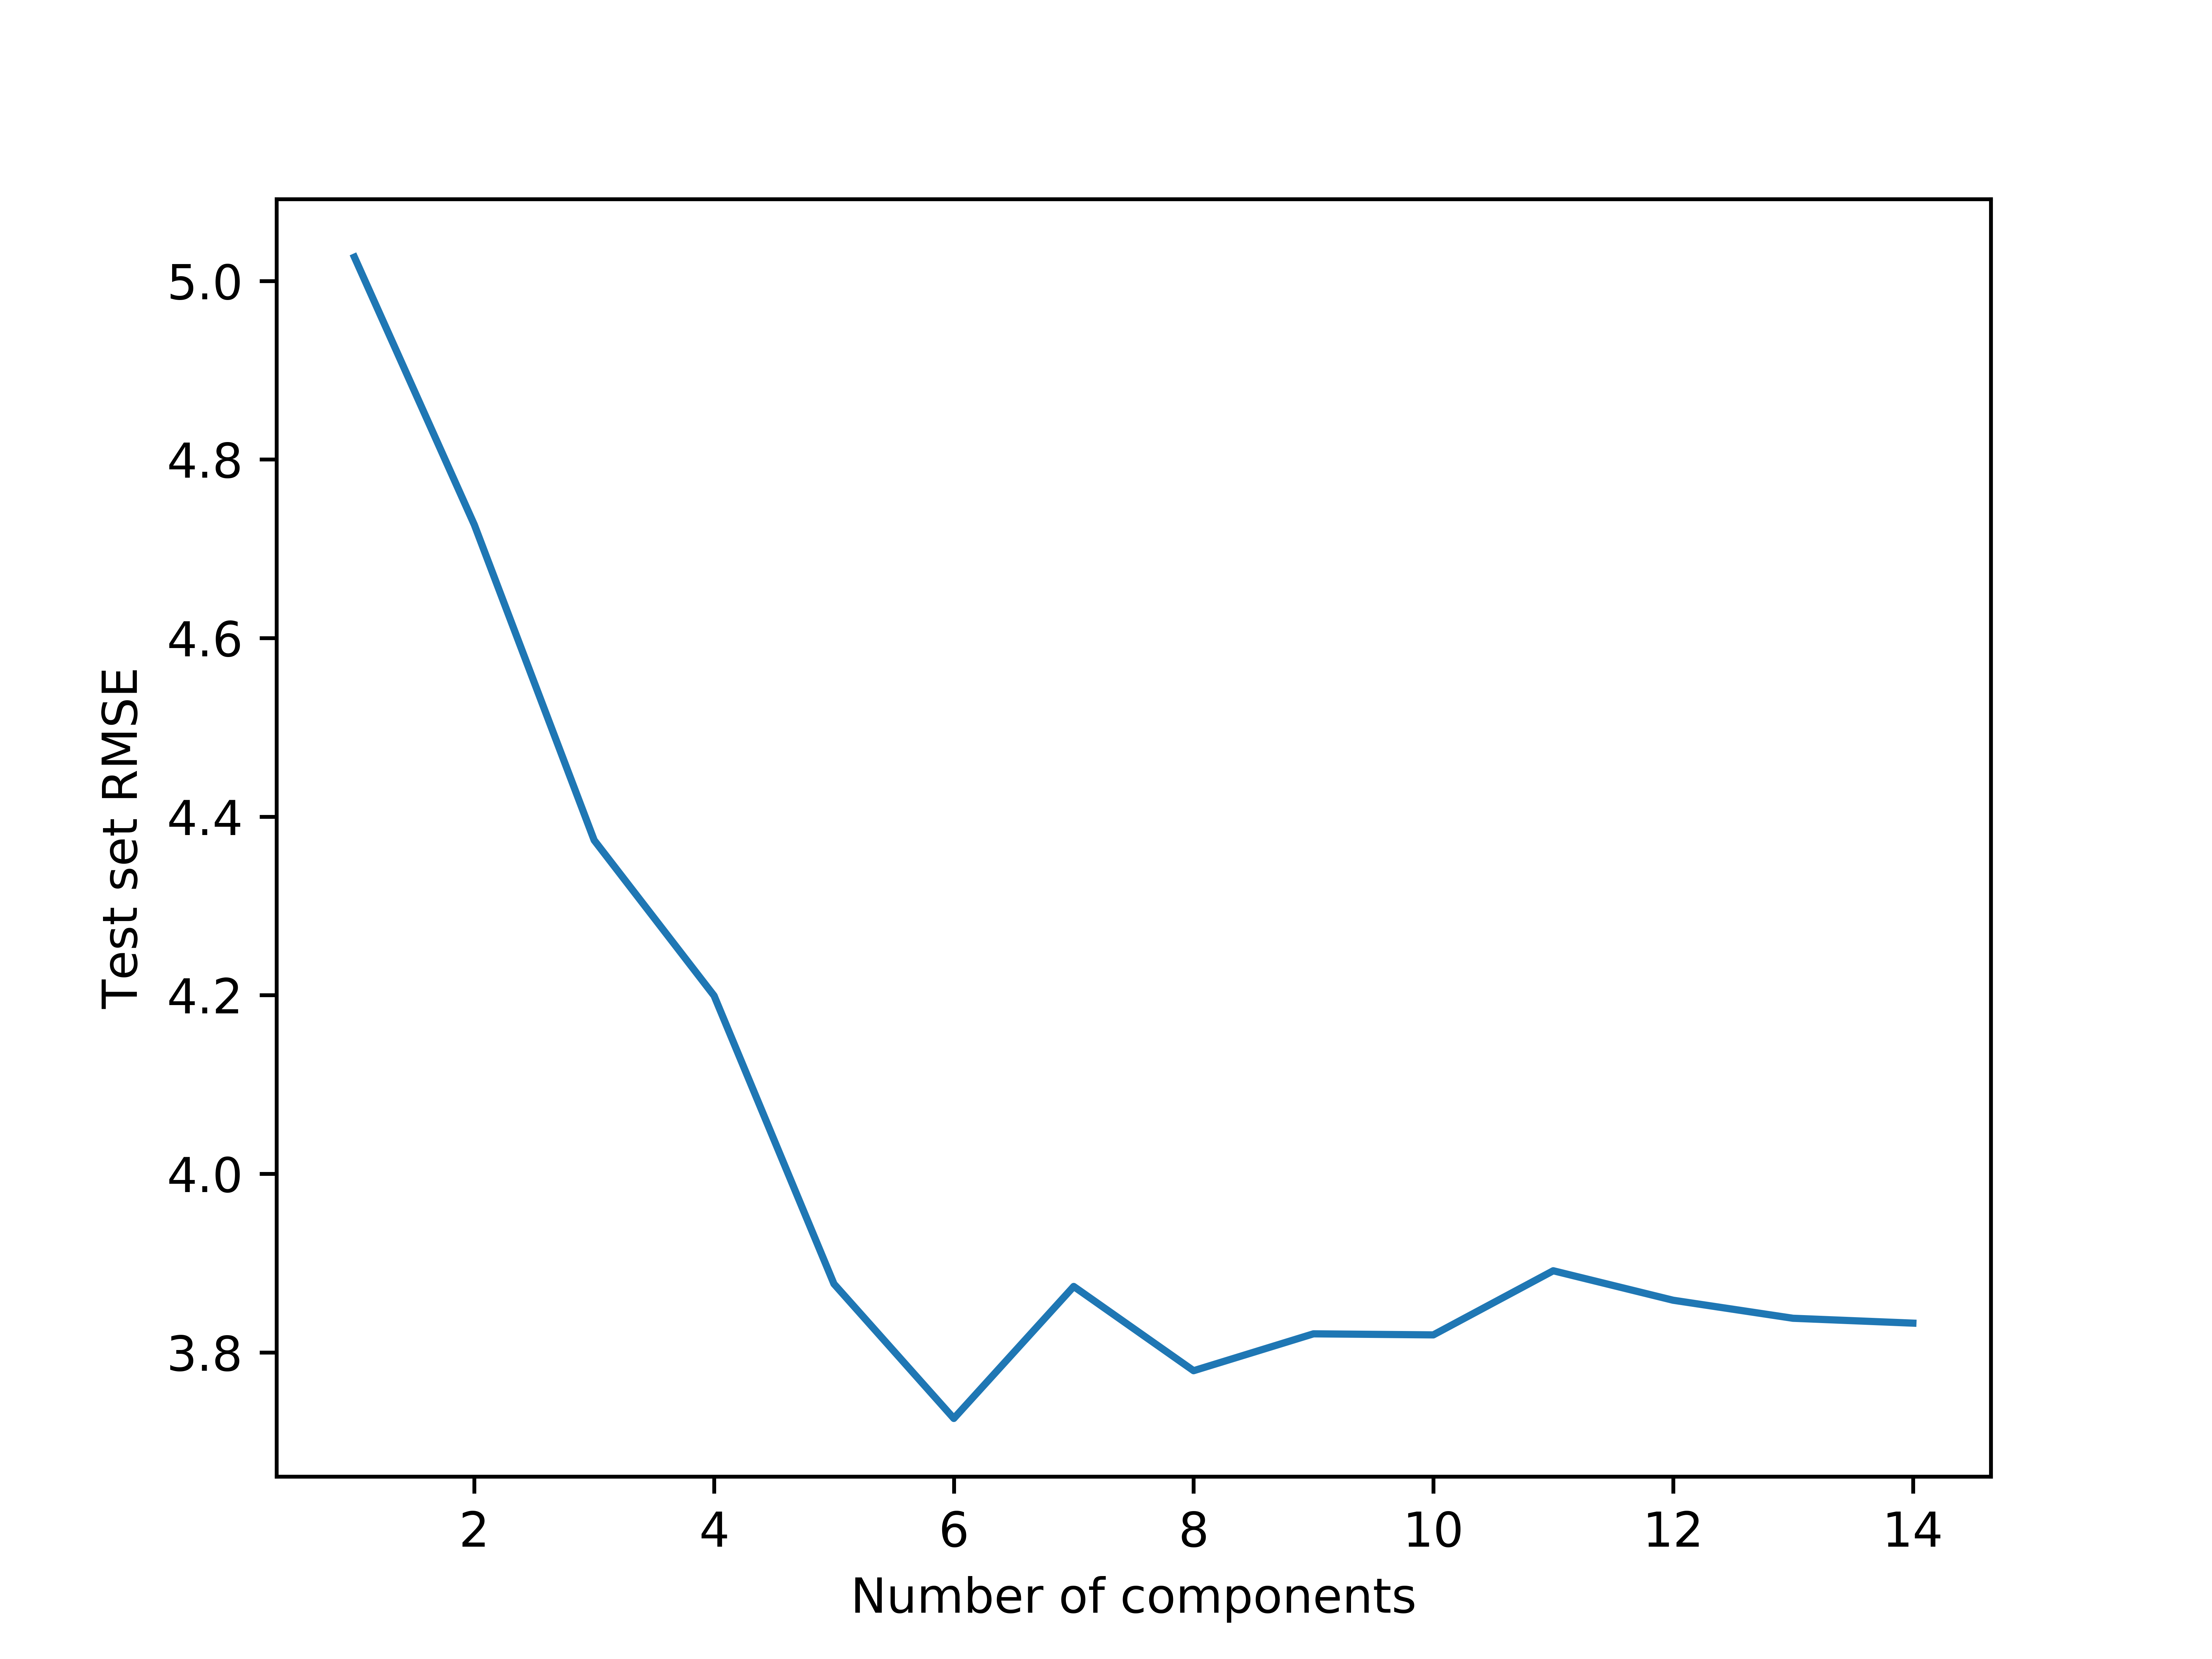
\includegraphics[width=0.48\textwidth]{rmse_vs_number_components}
	\caption{Performance of the partial least squares regression as a function of the number of latent variables. Training error always goes down since each additional component necessarily fits the residual data not explained by earlier components. Testing error reaches and then oscillates around a minimum value.\label{fig:rmse_vs_number_components}}
\end{center}
\end{figure}
\end{centering}

\begin{centering}
\begin{figure}
\centering
\begin{center}
	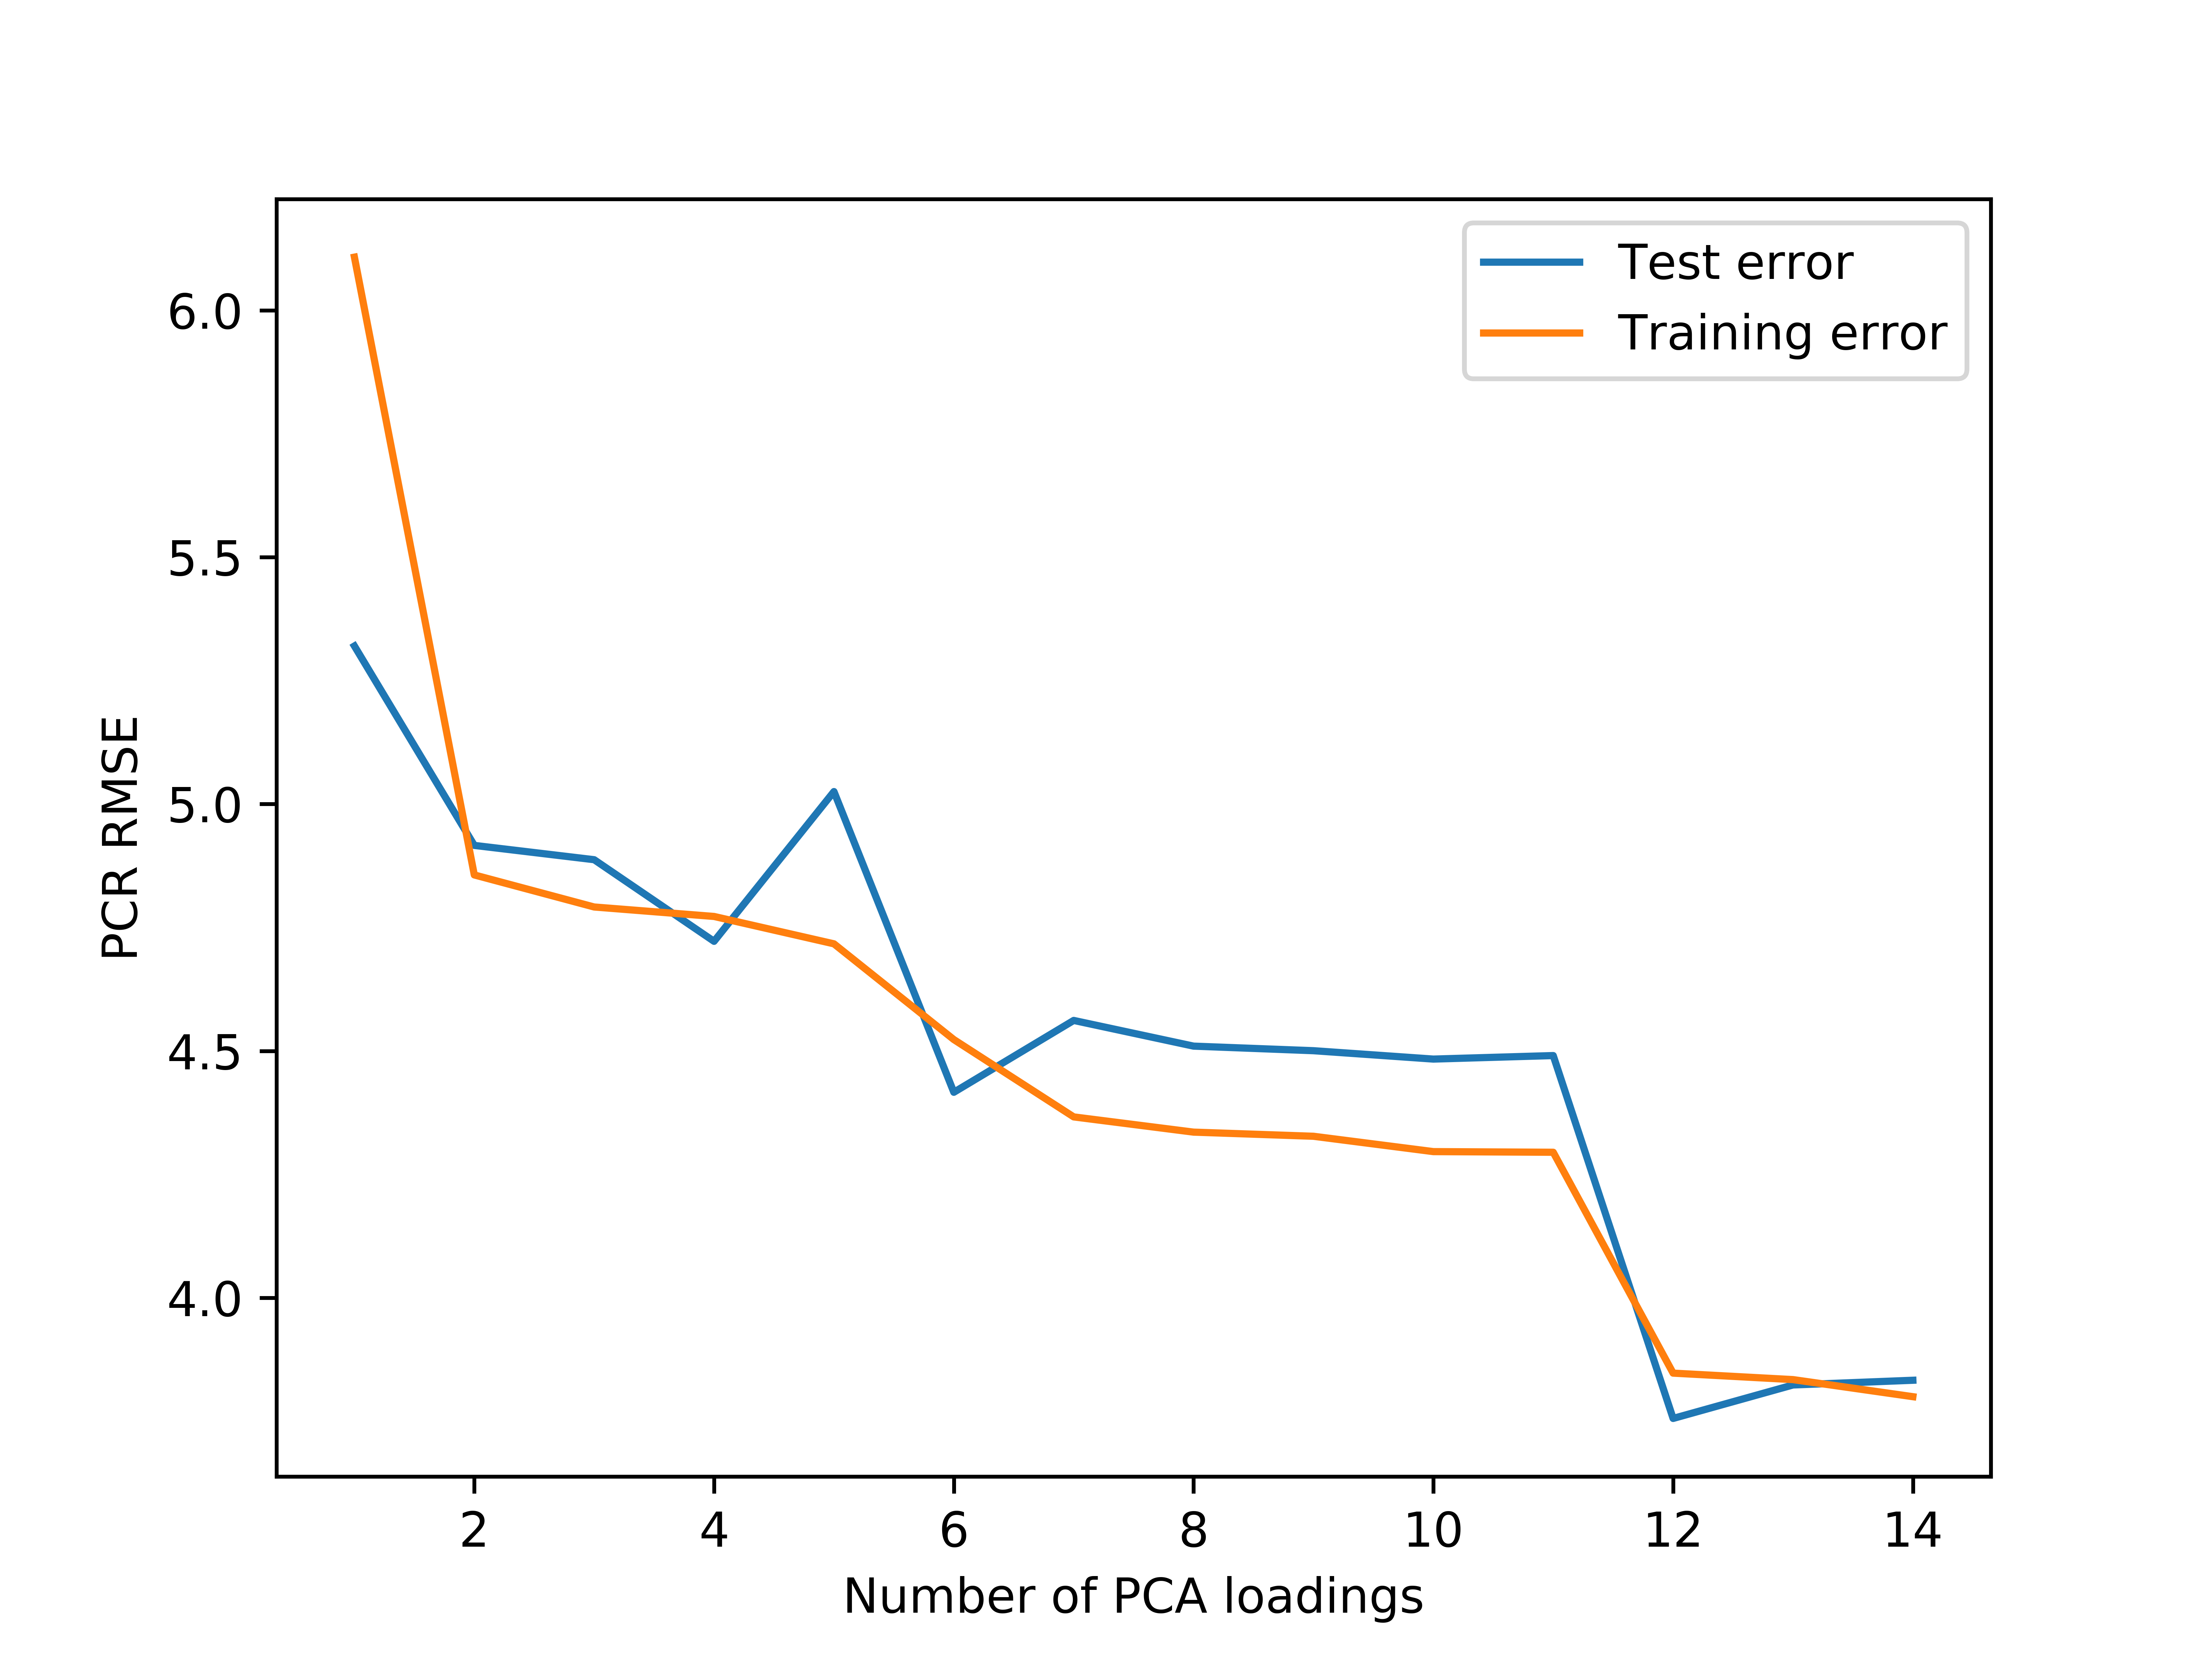
\includegraphics[width=0.48\textwidth]{rmse_vs_pca_loadings}
	\caption{Performance of the partial least squares regression as a function of the number of latent variables. Training error always goes down since each additional component necessarily fits the residual data not explained by earlier components. Testing error reaches and then oscillates around a minimum value.\label{fig:rmse_vs_pca_loadings}}
\end{center}
\end{figure}
\end{centering}

The difference between PLS latent variable weights and PCR is related to the supervised nature of PLS and the unsupervised nature of PCR. PCR loadings only capture the variance of the input data and are unaware of the output. The components are constructed to be purposefully orthogonal, unlike the PLS loadings. PLS latent variables are designed to capture the maximum possible covariance between $X_k$ and $y_k$, where $X_k, y_k$ are the residuals from the $(k-1)$th step. PLS latent variables are not necessarily orthogonal (though some algorithms do have this result, NIPALS does not).

The first four PLS weights and PCR components are shown in figure \ref{fig:pls_vs_pcr_loadings}. The first weight vector and component share some commonality (all values are positive, for example). Some similarity is to be expected as the first PCR loading was correlated with body fat percentage with a value of \num{0.64}. The second weight/component for each algorithm deviated more since the correlation of PC 2 was only \num{0.47}. Later PCs had a correlation with body fat of \num{0.1} or less; as expected, these showed no apparent relationship to the equivalent PLS weight vectors.

\begin{centering}
\begin{figure}
\centering
\begin{center}
	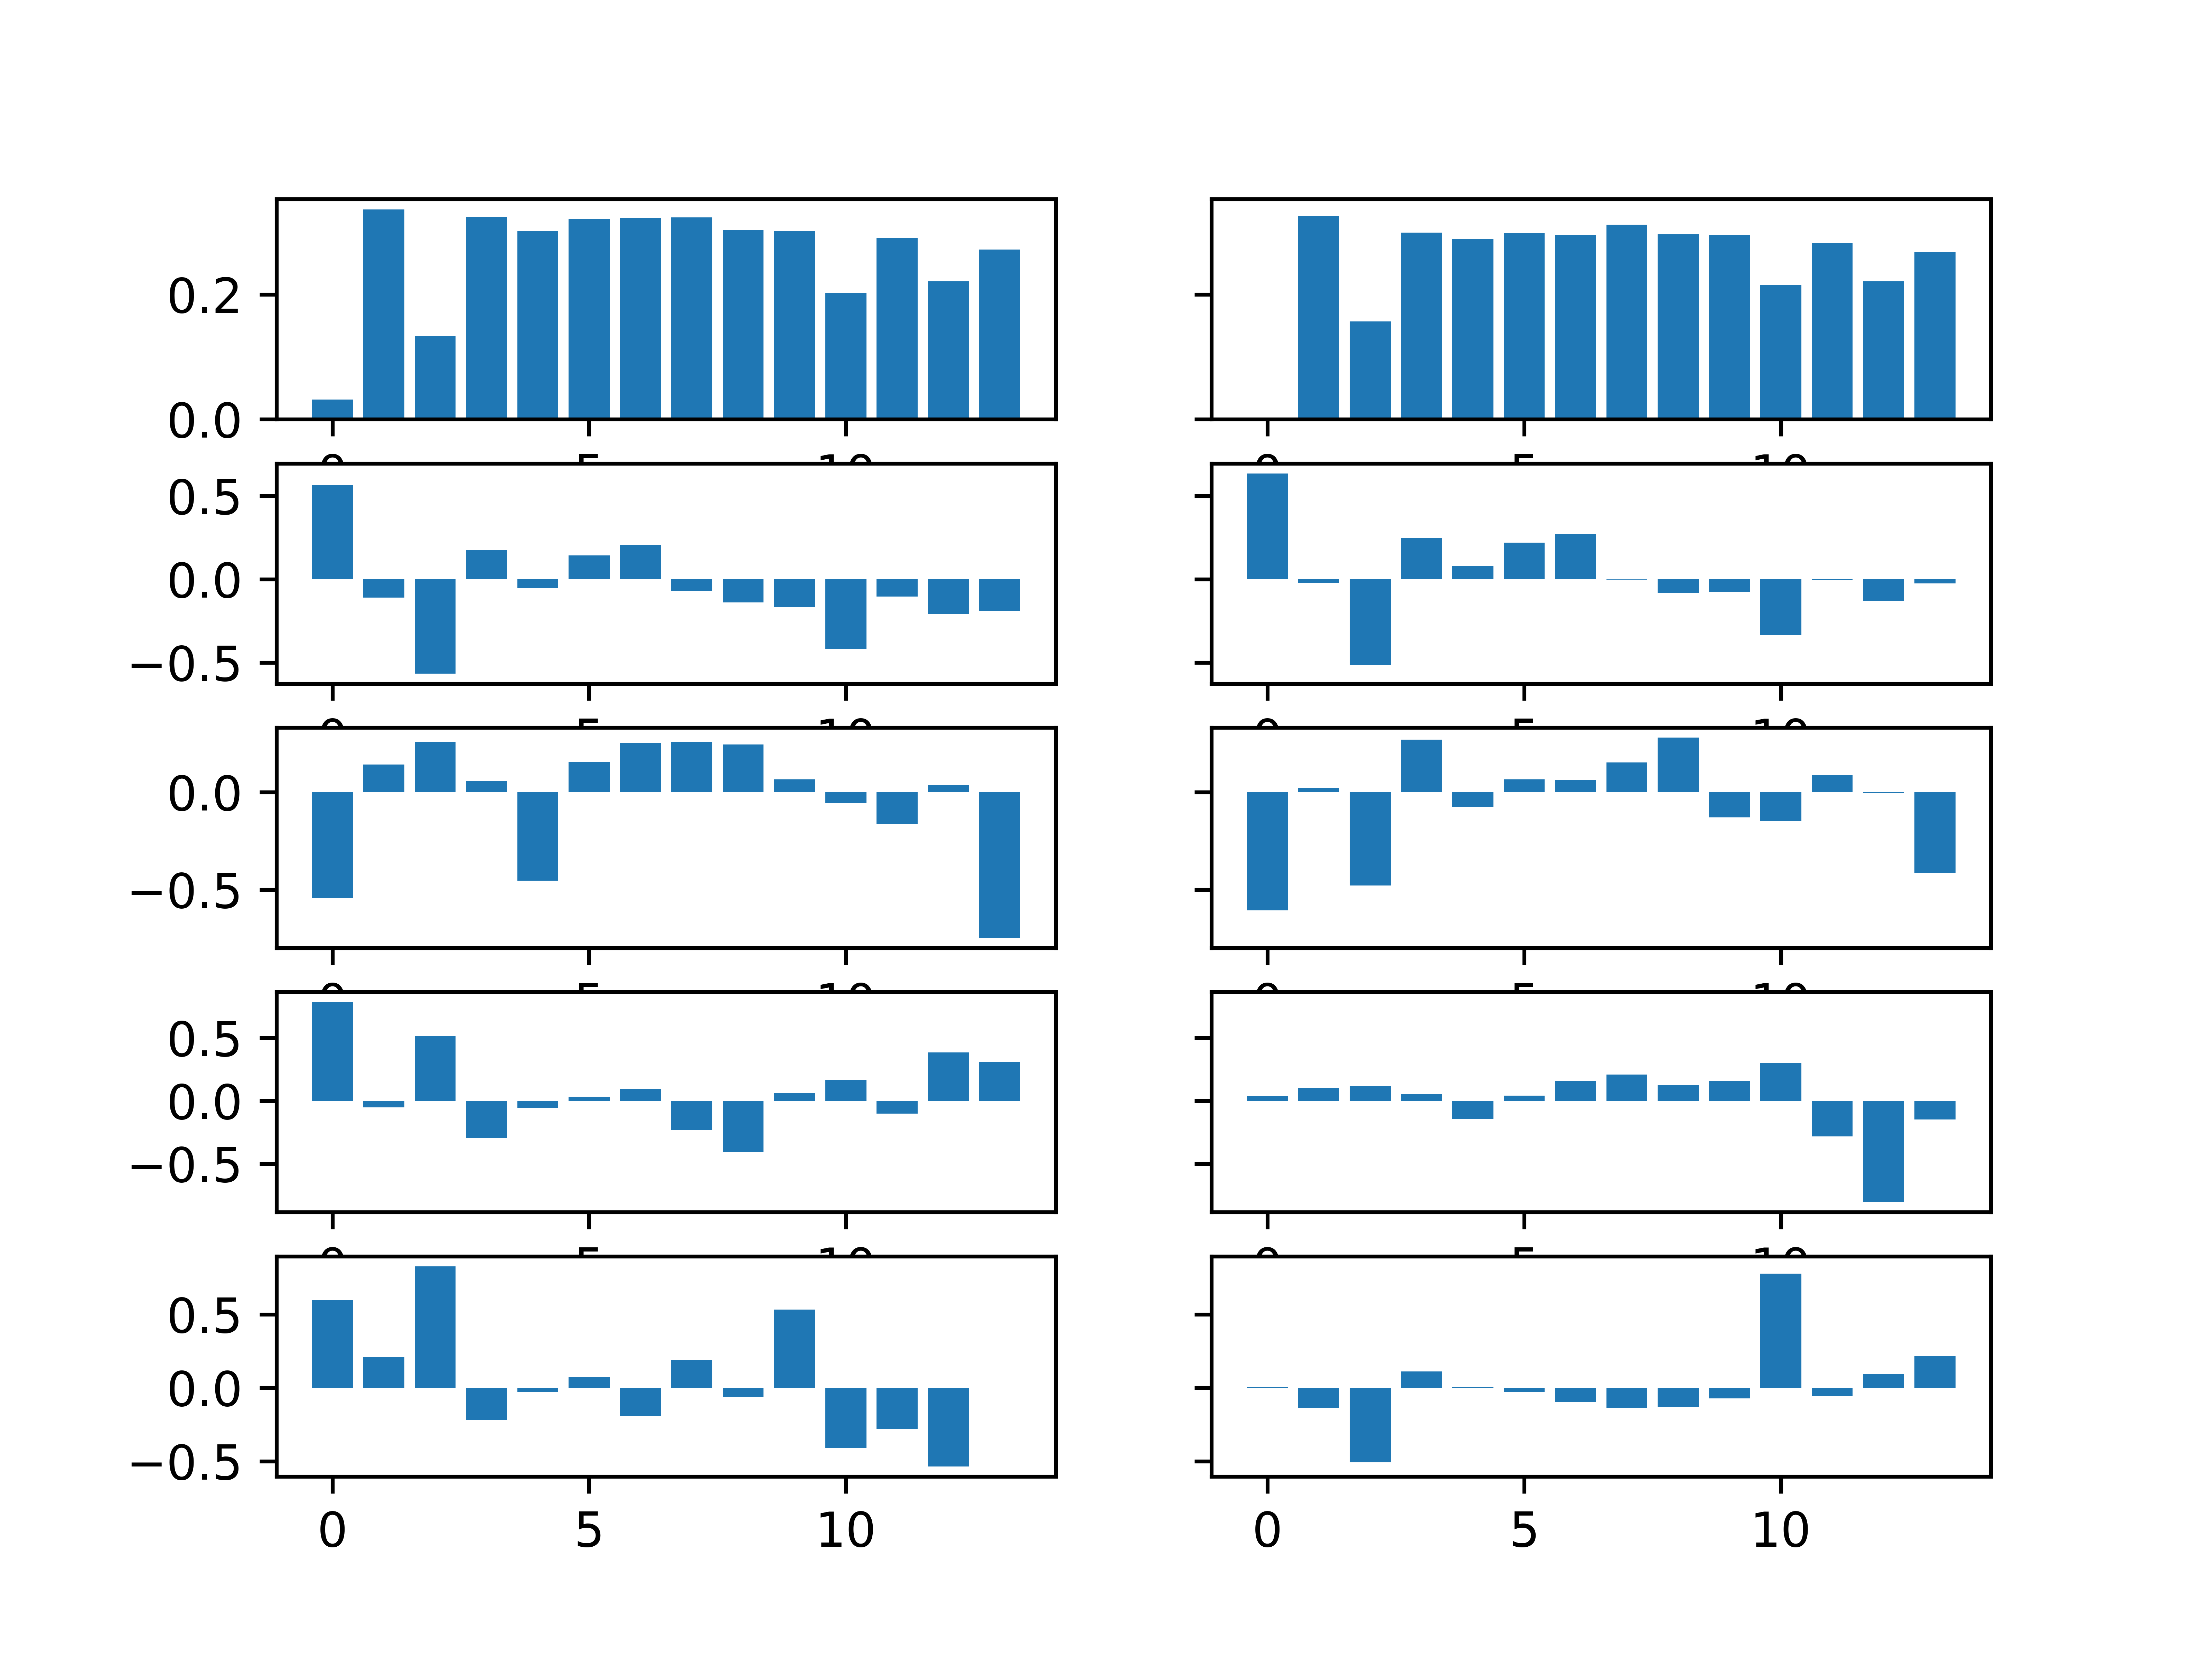
\includegraphics[width=0.48\textwidth]{pls_vs_pcr_loadings}
	\caption{Latent variable weights (left column) and PCR principal components (right column). The PLS weights differ from the principal components due to the supervised nature of PLS regression. PCR creates loadings based on variance in the input data while PLS creates weights based on covariance with output data.\label{fig:pls_vs_pcr_loadings}}
\end{center}
\end{figure}
\end{centering}

The weights of the first latent variable were compared to the correlation between the input and output variables (figure \ref{fig:pls_weights_and_correlation}). The two vectors were nearly identical, differing only in scale and the value corresponding to the height input variable. This is as expected--the first latent variable (LV 1) should be in the direction of maximum covariance with the output variable. Later latent variables (figure \ref{fig:first_four_latent_variables}) are designed to extend in the direction of the maximum covariance of the residual values of $\vec{y}$ once the contributions of earlier LV's are removed.

The first set of residuals of $\vec{y}$ (top right in figure \ref{fig:first_four_latent_variables}) appear the be primarily explained by the difference between age and height. The next largest contribution to LV 2 is ankle circumference. These three variables were the least correlated with body fat and were therefore the smallest contributors to LV 1. As such it makes sense that remaining correlations not captured by LV 1 are primarily in those variables.

\begin{centering}
\begin{figure}
\centering
\begin{center}
	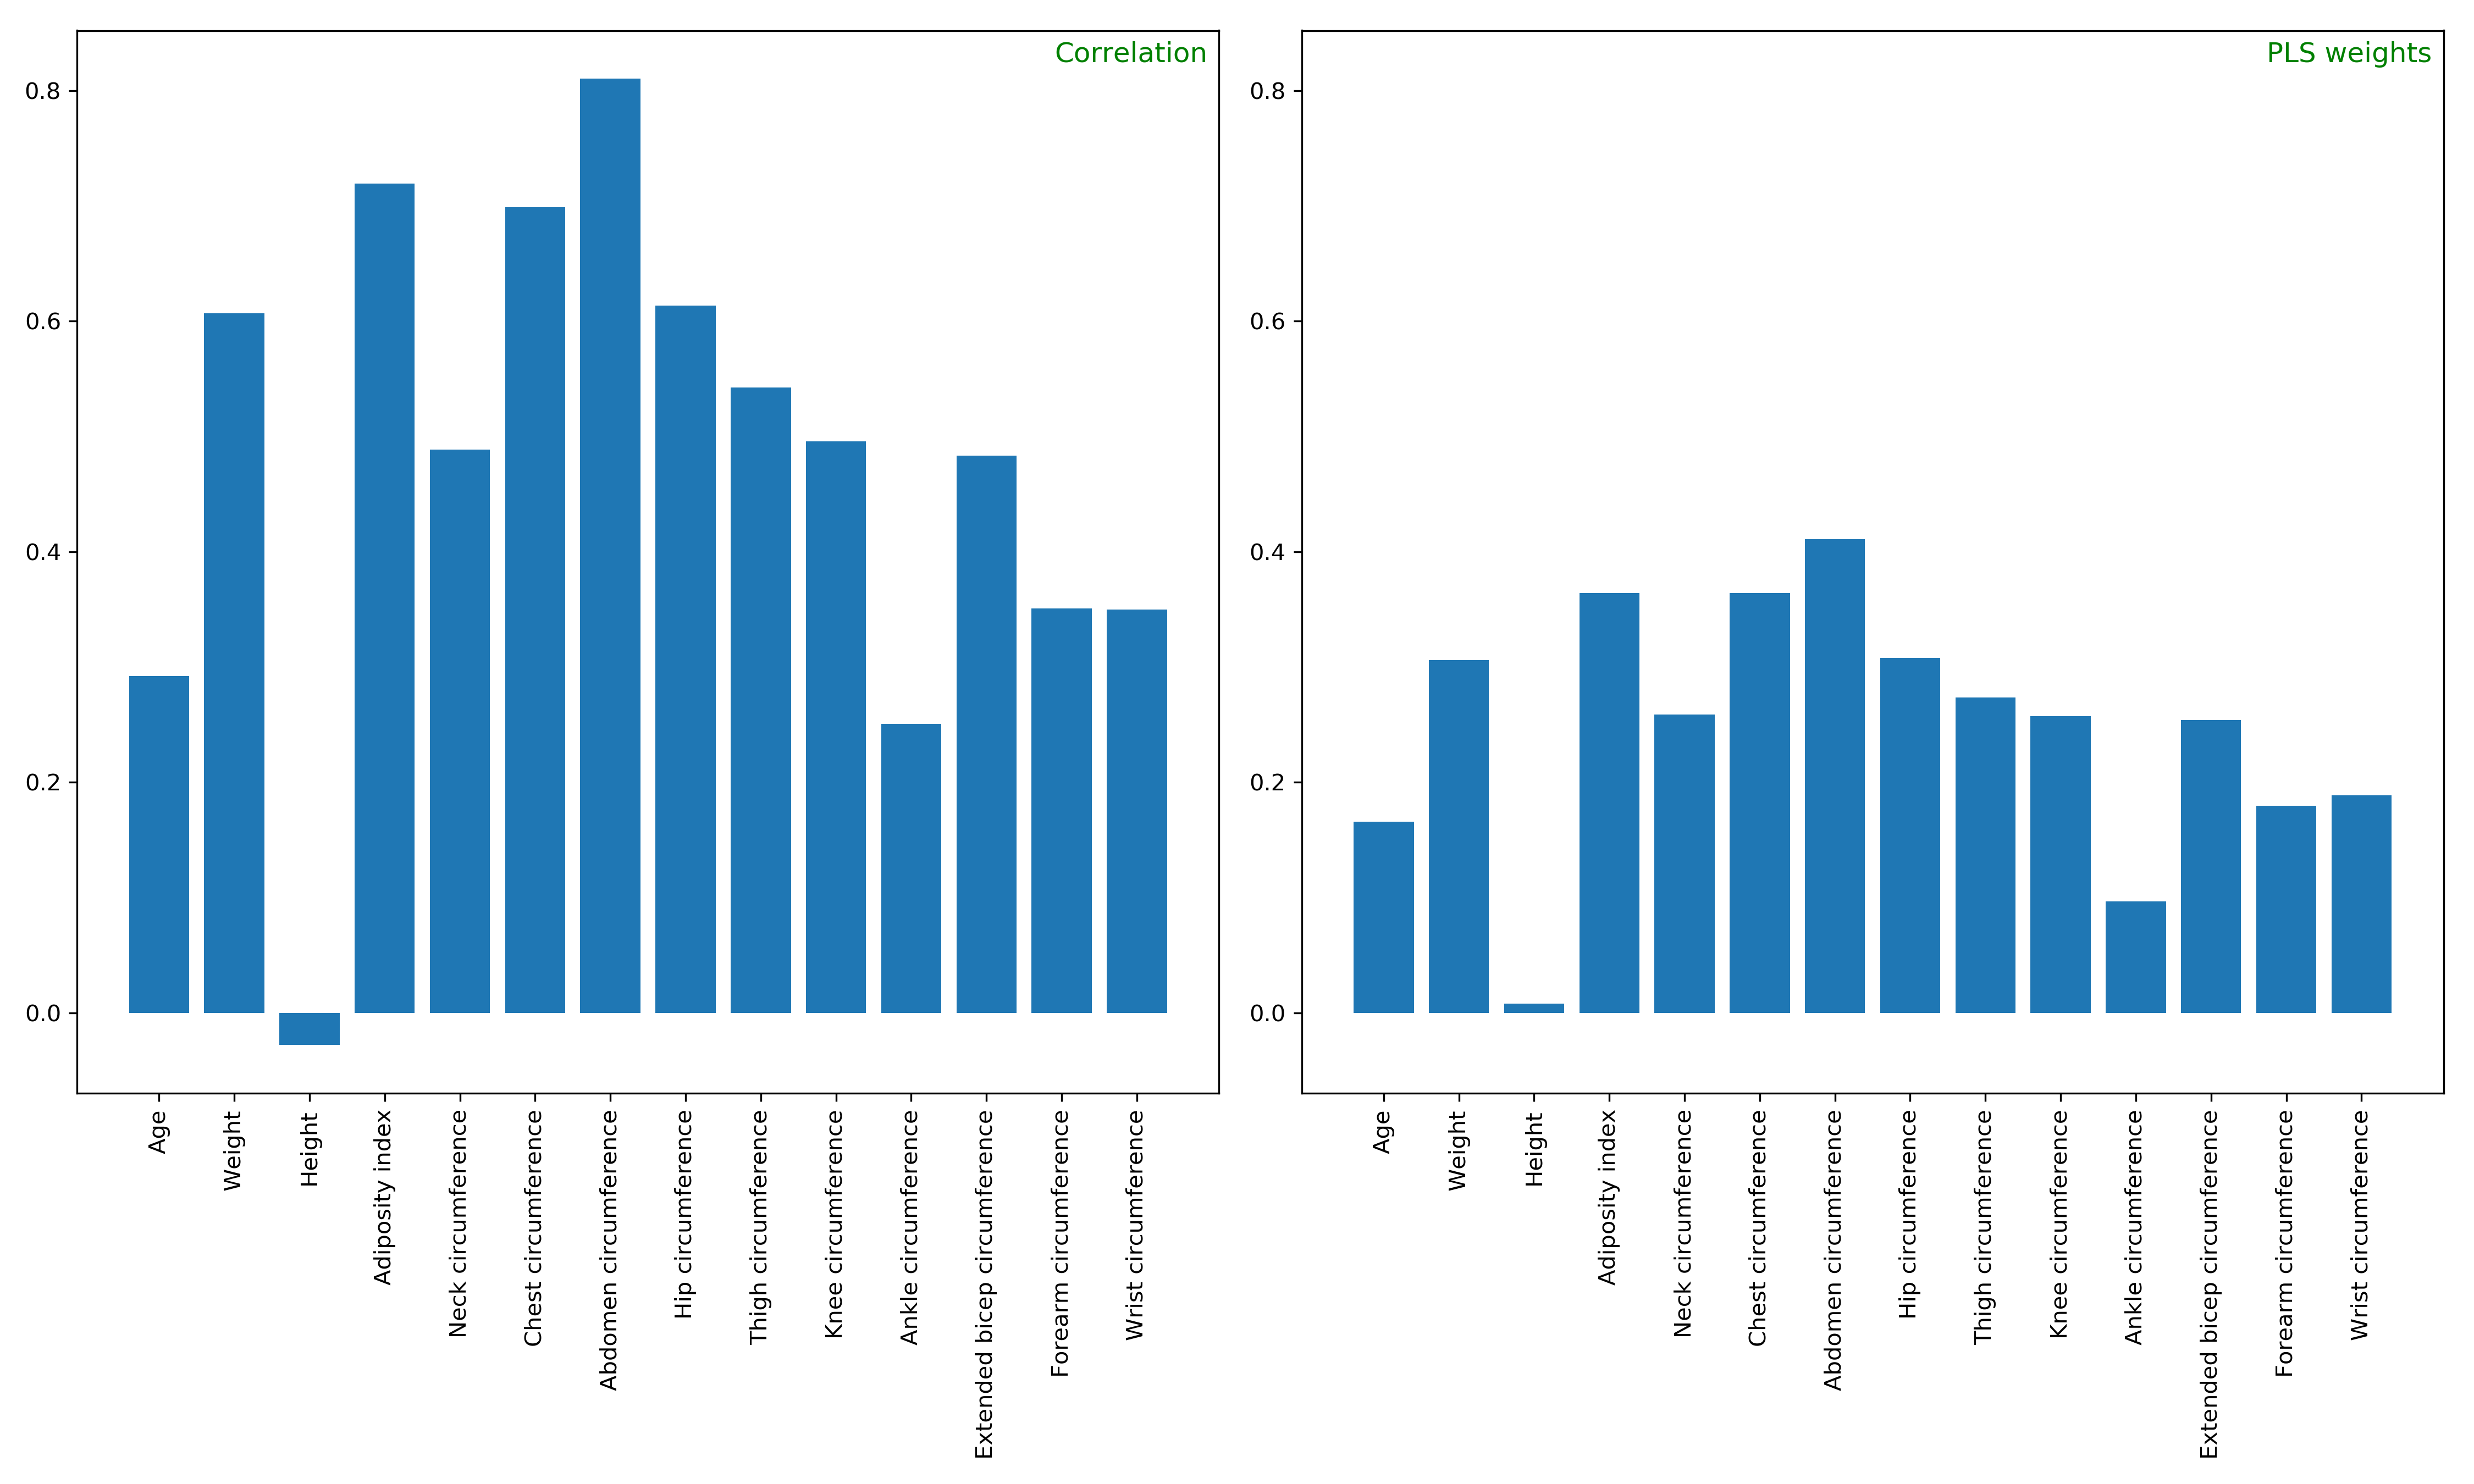
\includegraphics[width=0.48\textwidth]{pls_weights_and_correlation}
	\caption{The first latent variable weights (right) and correlation between the input matrix columns and outputs. While the scale is different, the two graphs clearly follow each other in form.\label{fig:pls_weights_and_correlation}}
\end{center}
\end{figure}
\end{centering}

\begin{centering}
\begin{figure}
\centering
\begin{center}
	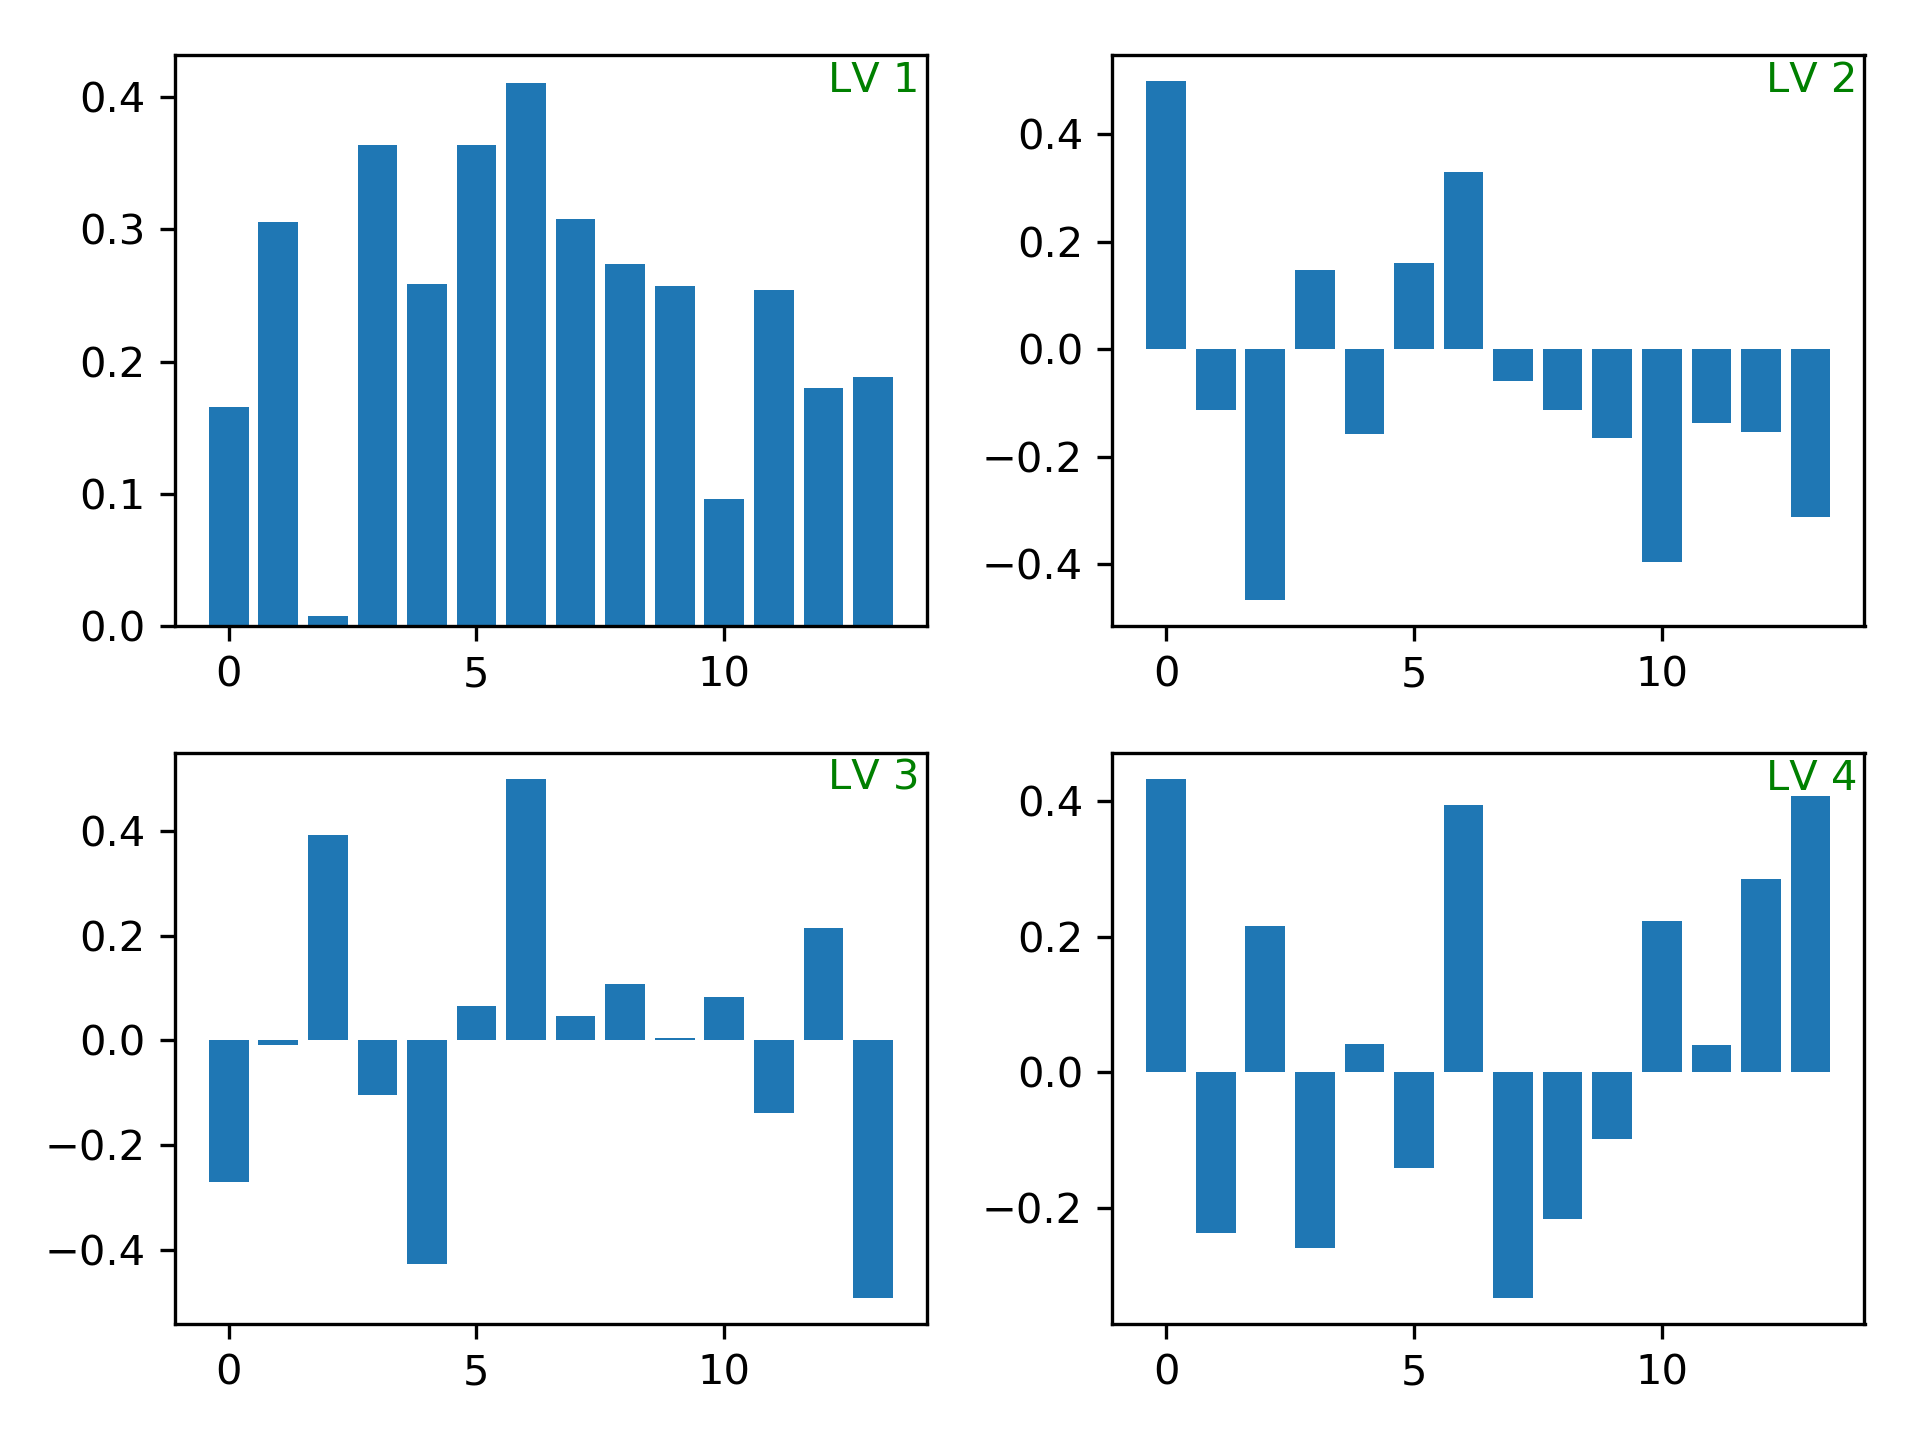
\includegraphics[width=0.48\textwidth]{first_four_latent_variables}
	\caption{The weights for the first four latent variables. Each weight is designed to translate the inputs into the direction corresponding to the maximum covariance with the residuals of the output.\label{fig:first_four_latent_variables}}
\end{center}
\end{figure}
\end{centering}

The selected model had six latent variables, corresponding to the minimum test set RMSE. The validation error for this model was \num{4.35}. This was lower than the error of the best principal component regression model (\num{4.72}) and the ``best guess'' linear regression model (\num{4.79}), but still not better than a linear regression using all inputs in the data set (\num{4.19}). Still, the improvement is significant and to be expected based on the supervised nature of the regression. Furthermore, the PLS model converged more quickly on the minimum error value with only \numrange{5}{6} latent variables required vice the $\approx\num{12}$ required from PCR. PCR also required additional analysis if non-consecutive loadings were used in the regression based on their correlation with the output. Since PLS latent variables are inherently ordered by covariance with the output model selection can be performed by a simple plot of test set error vs number of latent variables. Further, the PLS model outperformed the PCR model in spite of not having any polynomial or inverse terms added to it.

The possibility of using a nonlinear method to fit the $U$ and $T$ matrices was considered. Scatter plots of the X- and y- scores for the latent variables were generated (the first of these, for LV 1, is shown in figure \ref{fig:pls_first_scores_regression}). Since no apparent nonlinear relationship exists between the two scores, it was determined that a nonlinear PLS was not warranted in this instance. It did appear that one or more outliers might be affecting the linear fit. Future models may be implemented in such a way that an outlier rejection step is included before the regression step.

\begin{centering}
\begin{figure}
\centering
\begin{center}
	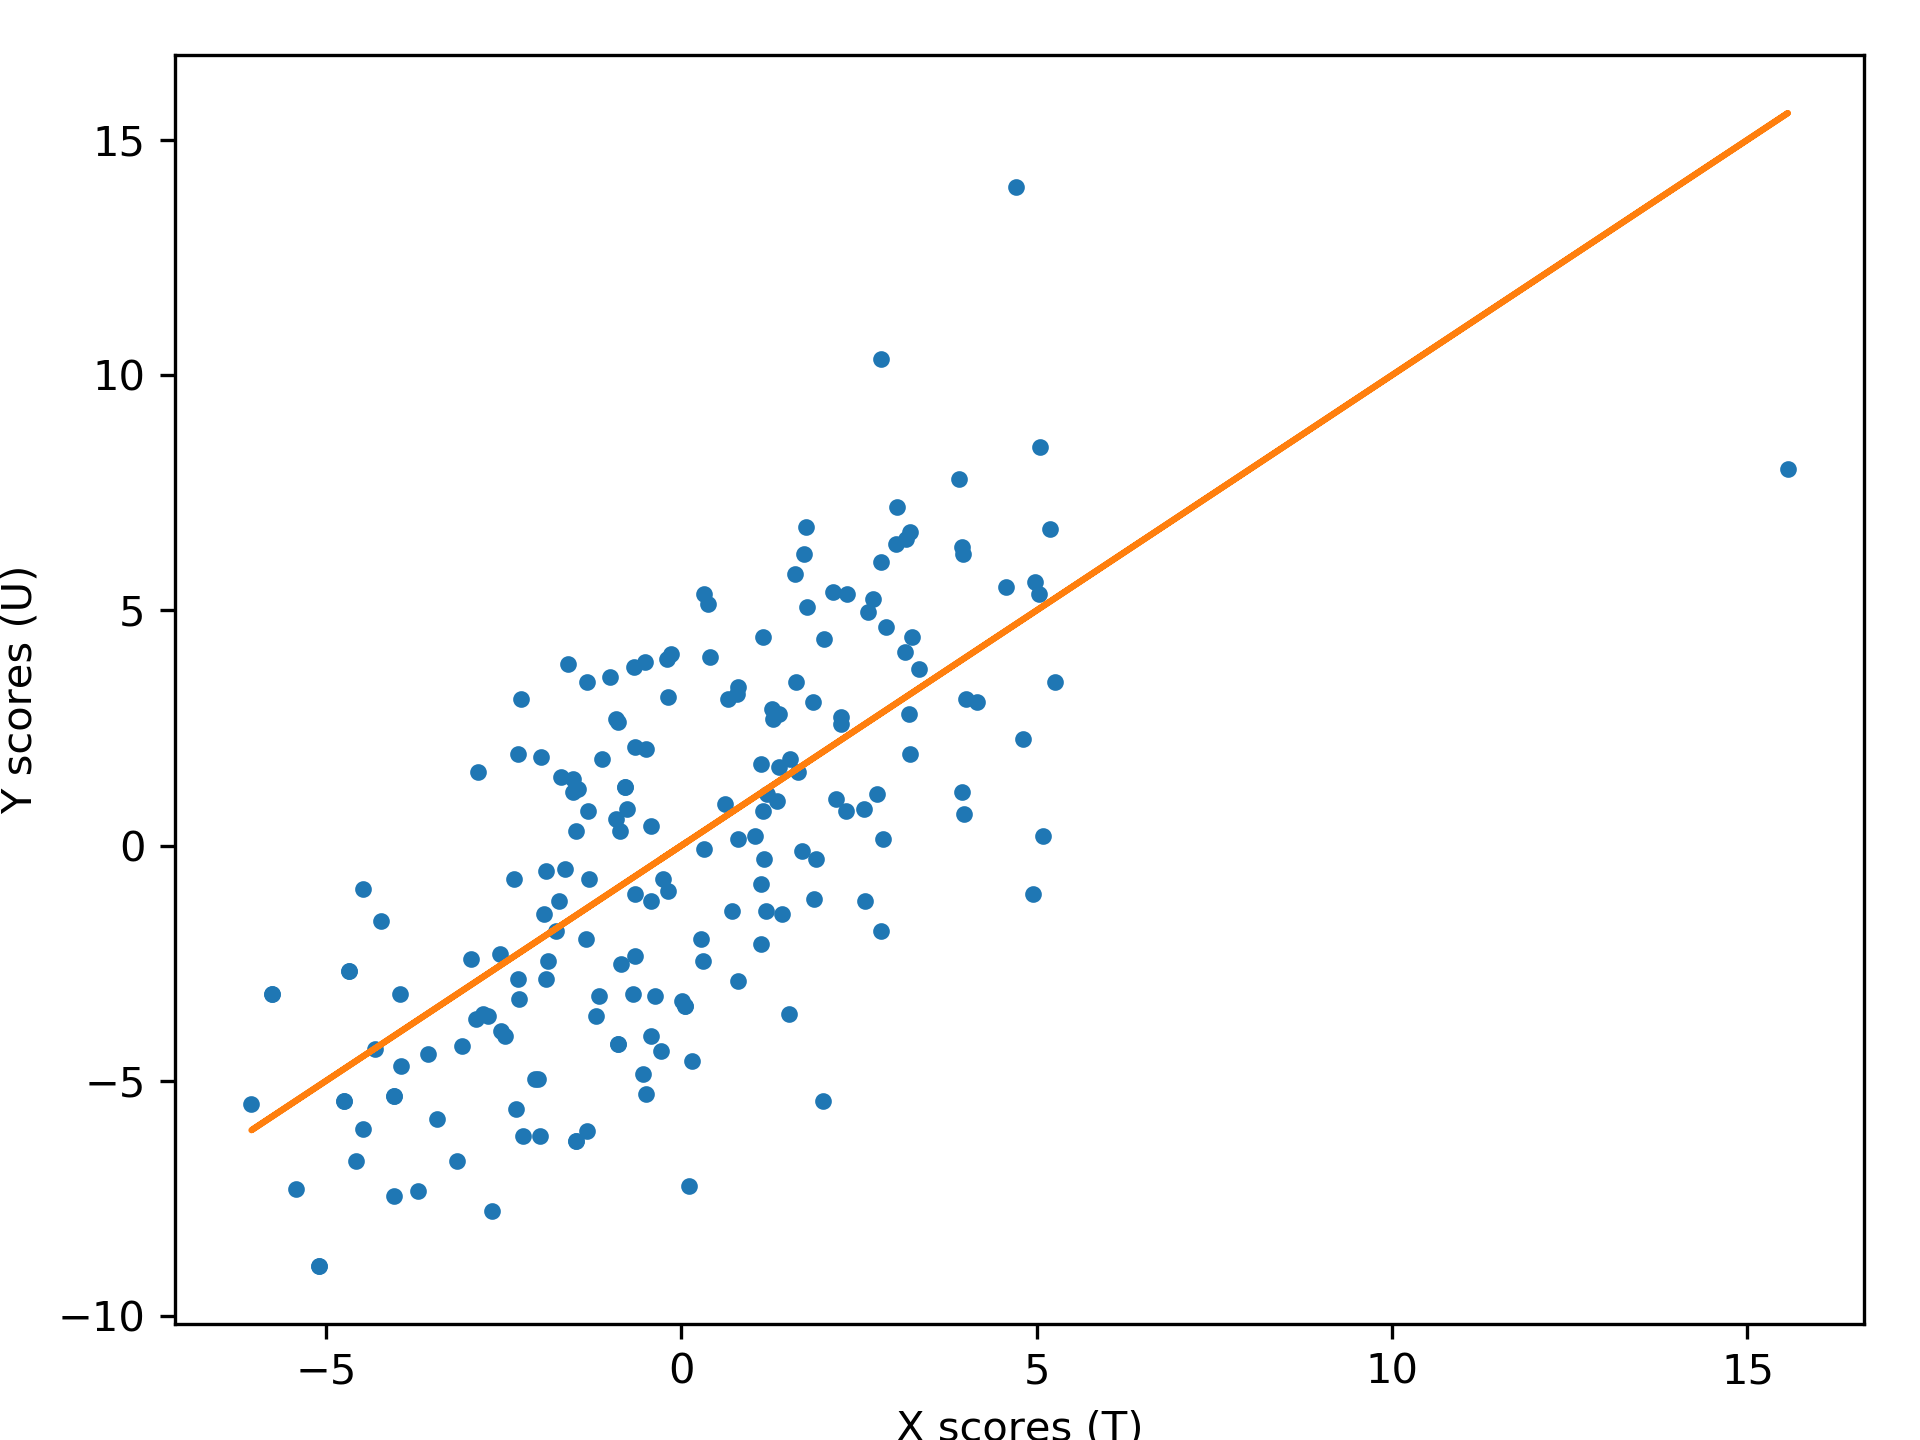
\includegraphics[width=0.48\textwidth]{pls_first_scores_regression}
	\caption{Regression between the X scores and Y scores for the first latent variable. No evidence of a nonlinear relationship was evident.\label{fig:pls_first_scores_regression}}
\end{center}
\end{figure}
\end{centering}

\section{Conclusions}

Partial least squares was used to generate a model that could predict body fat percentage with a root mean squared error of \num{4.35}. This outperformed models previously generated using linear regression and principal component regression even without the generation of polynomial, inverse, or interaction terms. PLS latent variables were compared to PCR principal components and determined to be fundamentally different in spite of the visual similarity. The smaller number of components required to minimize test set error was shown to be a natural result of selecting latent variables in order of maximum input/output covariance. This provides real-world advantages by simplifying model input and increasing the stability of models.

\printbibliography

\onecolumn
\section{Appendix}
Python code used to perform calculations and generate graphics.
\lstset{frame=single}
\lstinputlisting[language=python]{hw05.py}

\end{document}